\documentclass{article}
\usepackage{tikz}

\begin{document}

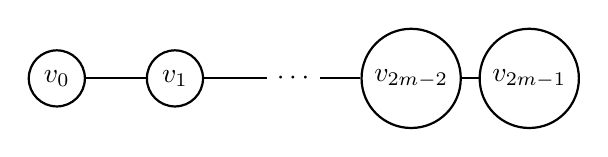
\begin{tikzpicture}[node distance={15mm}, thick, main/.style = {draw, circle}] 
    \node[main] (1) {$v_0$}; 
    \node[main] (2) [right of=1] {$v_1$}; 
    \node (3) [right of=2] {$\cdots$}; 
    \node[main] (4) [right of=3] {$v_{2m-2}$}; 
    \node[main] (5) [right of=4] {$v_{2m-1}$}; 

    \draw (1) -- (2); 
    \draw (2) -- (3); 
    \draw (3) -- (4); 
    \draw (4) -- (5); 
\end{tikzpicture}

The vertices \( v_1 \) through \( v_{2m-2} \) each have two neighbors, while \( v_0 \) and \( v_{2m-1} \) have one neighbor each. Thus, the vertices \( v_1 \) through \( v_{2m-2} \) have maximal degree for this graph.

\end{document}